\section{Motivación}
Interiorvista es una empresa especializada en la generación de imágenes por computador (mucho más baratas, rápidas y de igual o mejor calidad que las que pueden obtenerse con un plató y un fotógrafo) y en el desarrollo de aplicaciones web (que requieren personal muy especializado y una gran inversión de tiempo).

Entre estas aplicaciones se encuentran los \textit{Interiorvista Planner}, un conjunto de aplicaciones que tienen el objetivo de permitir a los usuarios generar habitaciones tridimensionales y poblarlas con los productos que los clientes ofrecen en su catálogo. Esto plantea una serie de retos a varios niveles.

En su estado actual, las aplicaciones desarrolladas tienen problemas que hacen cada vez más difícil el mantenimiento y la mejora de estas. Muchas de sus características han sido desarrolladas sin llevar a cabo ningún diseño previo, o incluso sin una especificación previa de los requerimientos de la aplicación, provocando que estos surjan a lo largo del desarrollo.

\begin{figure}[H]
    \centering
    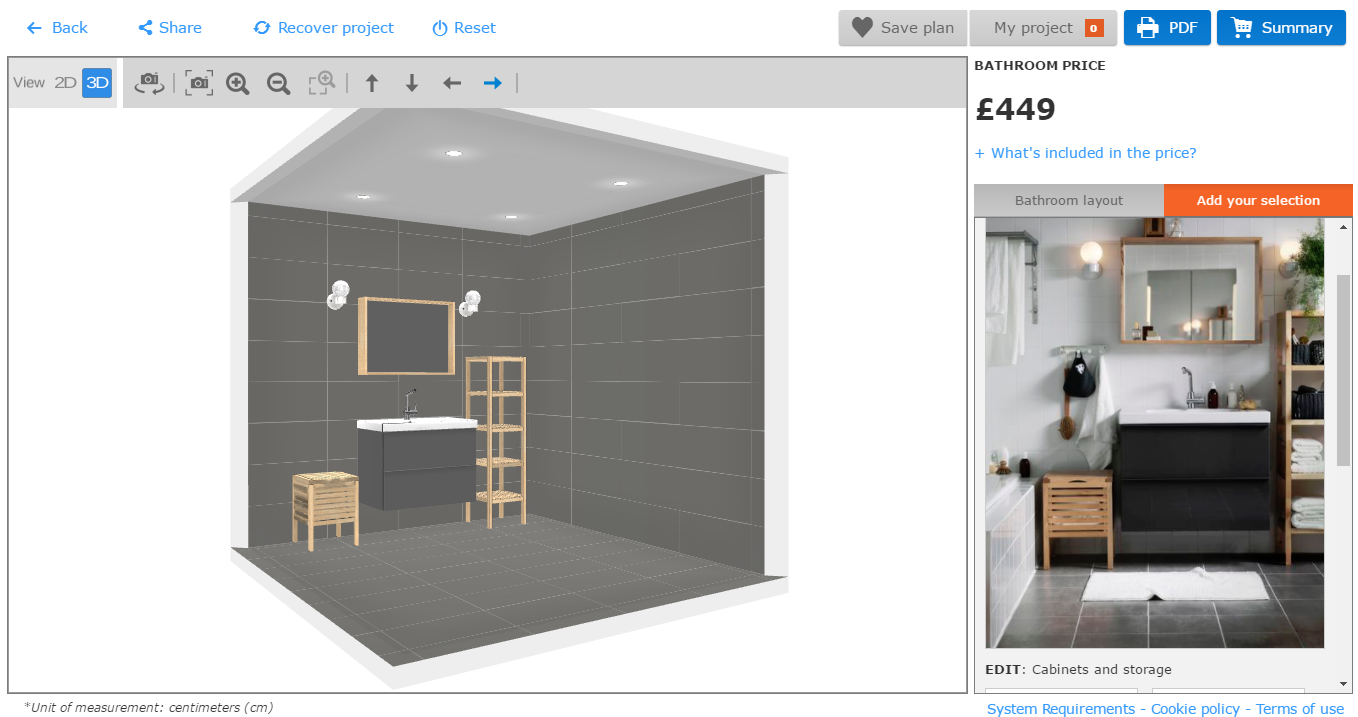
\includegraphics[width=0.8\linewidth]{bathroom_vista}
    \caption{Versión actual del planificador Bathroom Vista en vista 3D.}
    \label{fig:bathroom_vista}
\end{figure}


Las compañías de interiorismo suelen tener una serie de normas por las cuales ciertos elementos estructurales no pueden introducirse en ciertas combinaciones o en ciertas posiciones. Esto ha llevado a un código demasiado especializado en el que se introducen excepciones y condiciones arbitrarias sin mucho orden.

Se suelen requerir diversas aplicaciones muy similares para los distintos ambientes que ofrecen en su catálogo: habitaciones, comedores, baños, cocinas, etc. Aunque cada caso tiene sus particularidades, en general la mayoría de planificadores tienen suficientes características comunes como para poder tener un núcleo común, cosa que no está ocurriendo en estos momentos.

Generalmente casi siempre vamos a tener una habitación con ventanas, puertas, y una serie de elementos interiores que podemos distribuir por esta. Por ello, con un diseño efectivo debe ser posible reducir la especialización de cada una de estas aplicaciones. En el futuro, una posibilidad con la que se ha soñado en Interiorvista es la de hacer un planificador completo de una planta, con todas sus habitaciones, algo que no resultaría sencillo de conseguir con los desarrollos de que disponemos actualmente.

Entre las características comunes de los planificadores encontramos que la mayoría disponen de un modo visualización en 2 dimensiones, pensado para configurar la estructura de una habitación, y otro en 3 dimensiones, pensado para visualizar el resultado y realizar retoques sobre este. En estos momentos estos modos se han programado como dos programas distintos con una parte 2D hecha con tecnologías web, y una 3D hecha con un motor gráfico exportado a WebGL. Es una duplicidad de esfuerzos que puede evitarse utilizando una cámara ortogonal en 3D y algunas modificaciones visuales.

\begin{figure}[H]
    \centering
    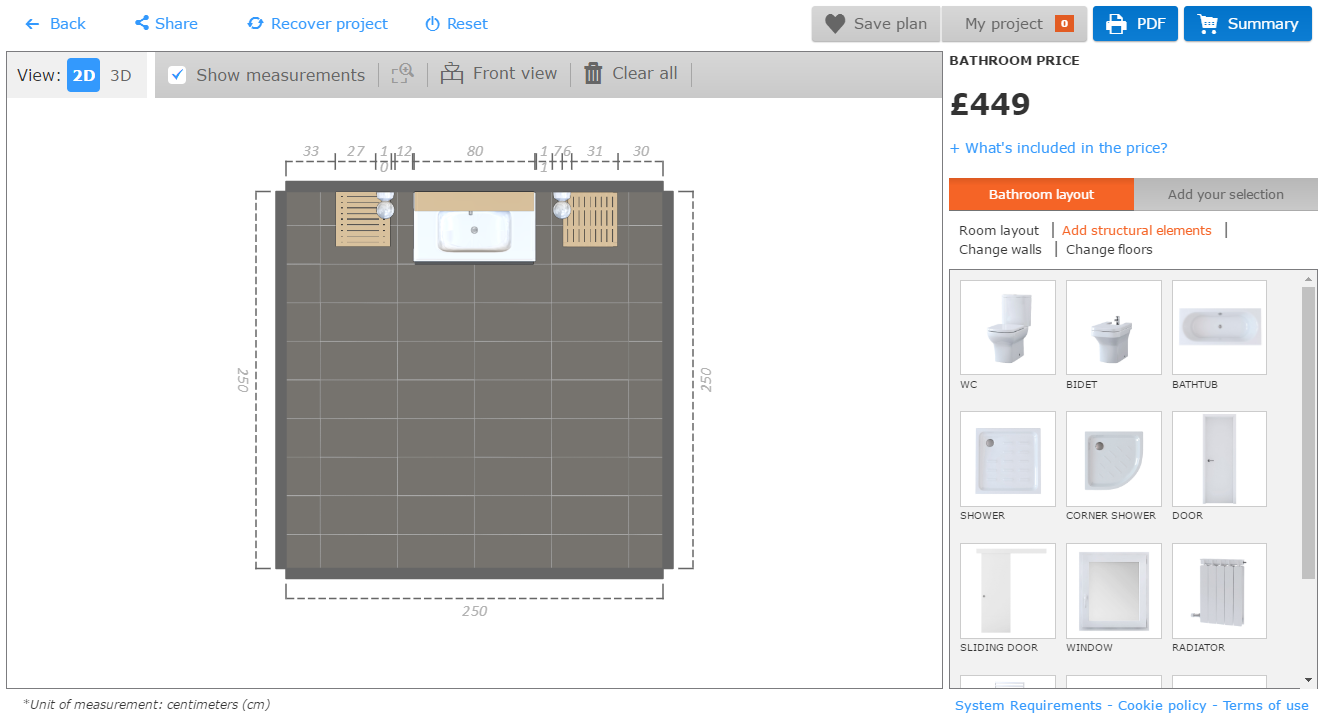
\includegraphics[width=0.8\linewidth]{bathroom_vista_2d}
    \caption{Bathroom Vista, versión en dos dimensiones del baño en la figura \ref{fig:bathroom_vista}.}
    \label{fig:bathroom_vista_2d}
\end{figure}

A pesar de las similitudes siempre hay elementos que hacen único a cada Planner: algunos baños o cocinas tienen diferentes texturas combinables para las paredes, algunas habitaciones tienen un techo inclinado o algunos productos de son altamente configurables y requieren más atención. Diferentes planificadores pueden tener un enfoque distinto: desde completas herramientas que han de poder generar y visualizar todas las configuraciones posibles de una estancia hasta aplicaciones que buscan un enfoque más emocional que atraiga a los usuarios, lo cual implica sacrificar funcionalidad en favor de la estética. Incluso pueden llegar a existir dos aplicaciones para un mismo conjunto de productos, con el objetivo de cubrir ambos puntos de vista.

El hecho de estar utilizando motores gráficos propietarios nos ha provocado problemas en el pasado. Las necesidades de la empresa son muy específicas y la imposibilidad de controlar el funcionamiento del motor ha hecho que no podamos solucionar efectivamente muchos problemas, llevándonos incluso a tener que esperar a que los desarrolladores lancen actualizaciones que arreglen nuestros problemas, o a mantener versiones abandonadas porque las versiones nuevas no son compatibles con ciertos requerimientos.

La falta de control sobre el motor gráfico también ha hecho que no pudiéramos realizar ciertas mejoras de eficiencia, visualización, o reducir el peso de la aplicación (por ejemplo, las versiones actuales incluyen toda una API de audio que no es necesaria).

\section{Objetivos}

La aplicación debe ser lo bastante genérica como para aplicarse a diferentes casos, de ahí que digamos que se trata de un conjunto de aplicaciones; y al mismo tiempo también ha de ser flexible como para dar cabida a todas estas características.

Debe contar con un visualizador en 2 y 3 dimensiones. Según el modo de visualización la interacción y las opciones son diferentes, pero el estado y la lógica de la aplicación debe mantenerse el máximo posible.

A largo plazo, la aplicación debe poder ejecutarse sobre distintas plataformas como web, escritorio, móviles o tabletas. Esto tiene muchas implicaciones a nivel de software e interacción: distintas plataformas cuentan con distintos drivers y APIs de ejecución y cada una tiene un funcionamiento y un modo de uso muy distinto. Dado que la aplicación va a estar completamente programada en C++, trasladar el código a otras plataformas (especialmente web) puede suponer un reto.

El desarrollo se realizará sobre un motor gráfico propio de la empresa, el cual está pensado para funcionar con la API gráfica Vulkan en escritorio, y debe ser adaptado para poder utilizarse con otras APIs en otras plataformas como Web o plataformas móviles. El hecho de disponer de un motor gráfico propio nos da un gran control sobre lo que ocurra dentro de este, en contraste con otras alternativas propietarias que no podemos controlar. En el pasado se han tenido muchos problemas haciendo funcionar las aplicaciones en distintas plataformas.

A nivel de diseño de software, esta es una oportunidad para repensar y reorganizar los problemas que ya conocemos. Aplicar correctamente diversas técnicas de diseño de software hará que no sólo sea más sencillo desarrollar la aplicación sino que sea más fácil de mantener y ampliar en el futuro. Algunas características son muy difíciles de implementar si no se ha seguido un cierto diseño desde el principio.

\section{Estado del arte}
Aunque existen diversos planificadores de estancias en el mercado, a día de hoy la mayoría tienen serias deficiencias y prácticamente ninguno está asociado a marcas importantes del modo en que lo está Interiorvista. Sin embargo, eso no impide que aprendamos de las alternativas existentes.

Entre los fallos más comunes se encuentran:
\begin{itemize}
    \item La necesidad de descargar aplicaciones de escritorio, o un gran número de assets que no necesariamente van a utilizarse.
    \item El uso de tecnologías obsoletas, especialmente Adobe Flash (muy popular durante la última década pero en desuso hoy en día), o motores web que requieren la instalación de plugins o extensiones.
    \item Sólo modo en 2 dimensiones o 3 dimensiones, sin la posibilidad de cambiar.
    \item Mala calidad gráfica.
    \item Interacción y/o diseño pobre.
\end{itemize}

Por supuesto, tenemos como precedente los anteriores planificadores hechos en Interiorvista, que aunque están bien situados en el mercado sufren de algunos de los fallos ya mencionados. La alternativa más sólida para lo que queremos realizar es Planner5D\footfullcite{planner5d}, que cumple buena parte de los requerimientos que queremos cumplir; sin embargo a día de hoy también tiene defectos en estabilidad e interacción, como que los elementos interiores no se adhieren a las paredes (a excepción de elementos estructurales de las paredes, como puertas y ventanas), o que en 2D pueden estropearse las paredes de forma relativamente fácil.

%Los planificadores de 2020\cite{2020} se caracterizan entre otras cosas por ofrecer imágenes estáticas de mayor calidad. El planificador espera a que el usuario deje de interactuar con la escena para generar la imagen y sobreponerla al canvas 3D. Aunque funciona, probablemente no se trata de la mejor aproximación a este problema, dado que el resultado no deja de ser un tanto pobre para la cantidad de trabajo que han realizado: generar un render 3D de buena calidad en la nube tiene un gran coste computacional (y por extensión, económico, pues los servidores gráficos son especialmente costosos), por lo que generar un render nuevo cada pocos segundos es inviable. Para solventarlo han reducido la calidad igualmente haciendo que, si bien se ve mejor que el render local, sigue dejando mucho que desear. Además, a nivel de interacción puede resultar engorroso notar el cambio de calidad constantemente.

%Generar imágenes de alta calidad en tiempo real no deja de ser una opción interesante, pero vale la pena considerar otras como mantener el renderizado local hasta que el usuario haya terminado de configurar su habitación, para finalmente generar una o varias imágenes de alta calidad.